\documentclass[UTF8,a4paper,8pt]{ctexart} 

\usepackage{graphicx}%学习插入图
\usepackage{verbatim}%学习注释多行
\usepackage{booktabs}%表格
\usepackage{geometry}%图片
\usepackage{amsmath}
\usepackage{amssymb}
\usepackage{listings}%代码
\usepackage{xcolor}  %颜色
\usepackage{enumitem}%列表格式
\setenumerate[1]{itemsep=0pt,partopsep=0pt,parsep=\parskip,topsep=5pt}
\setitemize[1]{itemsep=0pt,partopsep=0pt,parsep=\parskip,topsep=5pt}
\setdescription{itemsep=0pt,partopsep=0pt,parsep=\parskip,topsep=5pt}
\usepackage{tcolorbox}
\usepackage{algorithm}  %format of the algorithm
\usepackage{algorithmic}%format of the algorithm
\usepackage{multirow}   %multirow for format of table
\usepackage{tabularx} 	%表格排版格式控制
\usepackage{array}	%表格排版格式控制
\usepackage{hyperref} %超链接 \url{URL}

\CTEXsetup[format+={\flushleft}]{section}

%%%% 设置图片目录
\graphicspath{{figure/}}

%%%% 段落首行缩进两个字 %%%%
\makeatletter
\let\@afterindentfalse\@afterindenttrue
\@afterindenttrue
\makeatother
\setlength{\parindent}{2em}  %中文缩进两个汉字位

%%%% 下面的命令重定义页面边距,使其符合中文刊物习惯 %%%%
\addtolength{\topmargin}{-54pt}
\setlength{\oddsidemargin}{0.63cm}  % 3.17cm - 1 inch
\setlength{\evensidemargin}{\oddsidemargin}
\setlength{\textwidth}{14.66cm}
\setlength{\textheight}{24.00cm}    % 24.62

%%%% 下面的命令设置行间距与段落间距 %%%%
\linespread{1.4}
\setlength{\parskip}{0.5\baselineskip}
\geometry{left=1.6cm,right=1.8cm,top=2cm,bottom=1.7cm} %设置文章宽度
\pagestyle{plain} 		  %设置页面布局

%代码效果定义
\definecolor{mygreen}{rgb}{0,0.6,0}
\definecolor{mygray}{rgb}{0.5,0.5,0.5}
\definecolor{mymauve}{rgb}{0.58,0,0.82}
\lstset{ %
	backgroundcolor=\color{white},   % choose the background color
	basicstyle=\footnotesize\ttfamily,      % size of fonts used for the code
	%stringstyle=\color{codepurple},
	%basicstyle=\footnotesize,
	%breakatwhitespace=false,         
	%breaklines=true,                 
	%captionpos=b,                    
	%keepspaces=true,                 
	%numbers=left,                    
	%numbersep=5pt,                  
	%showspaces=false,                
	%showstringspaces=false,
	%showtabs=false,        
	columns=fullflexible,
	breaklines=true,                 % automatic line breaking only at whitespace
	captionpos=b,                    % sets the caption-position to bottom
	tabsize=4,
	commentstyle=\color{mygreen},    % comment style
	escapeinside={\%*}{*)},          % if you want to add LaTeX within your code
	keywordstyle=\color{blue},       % keyword style
	stringstyle=\color{mymauve}\ttfamily,     % string literal style
	frame=single,
	rulesepcolor=\color{red!20!green!20!blue!20},
	% identifierstyle=\color{red},
	language=c++,
}
 \author{\kaishu 郑华}
 \title{游戏服务器 笔记}

\begin{document}          %正文排版开始
 	\maketitle
\newpage
  
\section{弱交互游戏服务端}

	\subsection{用户特点}
		\begin{enumerate}[fullwidth,itemindent = 2em]
			\item  交互弱
			\item  不需要实时PK
			\item  利用本地数据进行游戏(离线数据)
		\end{enumerate}
		
		故采用Http服务器。
     
	    \begin{figure}[h] 	
	    	\centering
	    	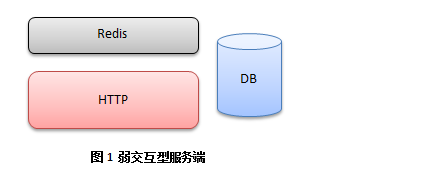
\includegraphics[width=8cm,clip]{weakServer.png} 	
	    	\label{fig:weakServer}
	    \end{figure} 
	    
	 \subsection{具体细节}
		 \paragraph{登陆}登录时可以使用非对称加密(RSA, DH),服务器根据客户端uid,当前时间戳还有服务端私钥,计算哈希得到的加密 key 并发送给客户端。之后双方都用 HTTP通信,并用那个key进行RC4加密。客户端收到key和时间戳后保存在内存,用于之后通信,服务端不需要保存 key,因为每次都可以根据客户端传上来的 uid 和 时间戳 以及服务端自己的私钥计算得到。用模仿 TLS的行为,来保证多次 HTTP请求间的客户端身份,并通过时间戳保证同一人两次登录密钥不同。
    
	    \paragraph{对局}每局开始时,访问一下,请求一下关卡数据,玩完了又提交一下,验算一下是否合法,获得什么奖励,数据库用单台 MySQL或者 MongoDB即可,后端的 Redis做缓存(可选)。如果要实现通知,那么让客户端定时15秒轮询一下服务器,如果有消息就取下来,如果没消息可以逐步放长轮询时间,比如30秒;如果有消息,就缩短轮询时间到10秒,5秒,即便两人聊天,延迟也能自适应。
	    
	 \subsection{总结} 此类服务器用来实现一款三国类策略或者卡牌及酷跑的游戏已经绰绰有余,这类游戏因为逻辑简单,玩家之间交互不强,使用 HTTP来开发的话,开发速度快,调试只需要一个浏览器就可以把逻辑调试清楚了。
\newpage
\section{Mudos 游戏服务器}
		\subsection{用户特点}
			\begin{enumerate}[fullwidth,itemindent = 2em]
				\item  玩家和玩家之间有比较强的交互(聊天,交易,PK)
				\item  需要实时PK
				\item  利用在线数据进行游戏
			\end{enumerate}
			
			\begin{figure}[h] 	
				\centering
				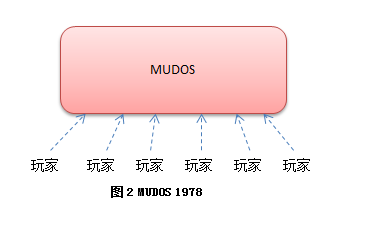
\includegraphics[width=8cm,clip]{gameServer2.png} 	
				\label{fig:gameServer2}
			\end{figure} 
	   \subsection{具体细节}
		  
			\paragraph{交互}MUDOS使用单线程无阻塞套接字来服务所有玩家,所有玩家的请求都发到同一个线程去处理,主线程每隔1秒钟更新一次所有对象(网络收发,更新对象状态机,处理超时,刷新地图,刷新NPC)。
			
			用户使用 Telnet之类的客户端用 Tcp协议连接到 MUDOS上,使用纯文字进行游戏,每条指令用回车进行分割。
			
			\paragraph{数据保存}用户数据保存在文件中,每个用户登录时,从文本文件里把用户的数据全部加载进来,操作全部在内存里面进行,无需马上刷回磁盘。用户退出了,或者每隔5分钟检查到数据改动了,都会保存会磁盘。这样的系统在当时每台服务器承载个4000人同时游戏,不是特别大的问题。MUDOS发布后,全球各地都在为他改进,扩充,退出新版本,随着 Windows图形机能的增强。游戏《UO》在 MUDOS的基础上为角色增加的x,y坐标,为每个房间增加了地图,并且为每个角色增加了动画,形成了第一代的图形网络游戏。
			
			\paragraph{服务端引擎概念}因为游戏内容基本可以通过 LPC脚本进行定制,所以MUDOS也成为名副其实的第一款服务端引擎,引擎一次性开发出来,然后制作不同游戏内容。后续国内的《万王之王》等游戏,很多都是跟《UO》一样,直接在 MUDOS上进行二次开发,加入房间的地图还有角色的坐标等要素,该架构一直为国内的第一代 MMORPG提供了稳固的支持.
			
	\subsection{总结}虽然是一个架构,但是它会随游戏内容的复杂程度,架构变得吃不消,所以现在并不流行。
\newpage	
\section{数据库服务器时代}
		\subsection{用户特点}
			\begin{enumerate}[fullwidth,itemindent = 2em]
				\item  频繁的读取数据
				\item  在线人数多
				\item  利用在线数据进行游戏
			\end{enumerate}
	    \subsection{演变}	
			\paragraph{引入数据库}早期 EXT磁盘分区比较脆弱,断电容易发生大面积数据丢失。因此第一步就是拆分文件存储到数据库,如图3。
			
			\begin{figure}[h] 	
				\centering
				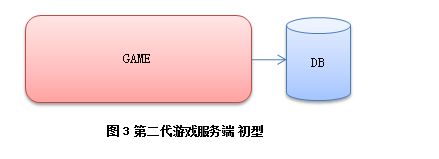
\includegraphics[width=8cm,clip]{gameServer3.png} 	
				\label{fig:gameServer3}
			\end{figure} 
			
			\paragraph{拆分游戏世界}随着游戏内容的增加,传统单服务器的结构进一步成为瓶颈。于是有人开始拆分游戏世界,变为下面的模型,如图4:
			
			\begin{figure}[h] 	
				\centering
				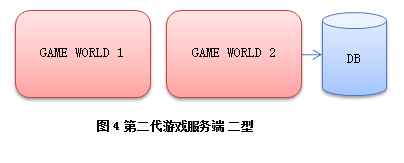
\includegraphics[width=8cm,clip]{gameServer4.png} 	
				\label{fig:gameServer4}
			\end{figure} 
			
			\paragraph{解决数据库瓶颈问题}游戏服务器压力拆分后得意缓解,但是两台游戏服务器同时访问数据库,大量重复访问,大量数据交换,使得数据库成为下一个瓶颈。于是形成了数据库前端代理(DB Proxy),游戏服务器不直接访问数据库而是访问代理,再有代理访问数据库,同时提供内存级别的cache,如图5.
			
			\begin{figure}[h] 	
				\centering
				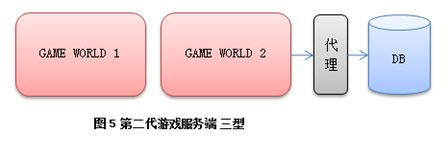
\includegraphics[width=8cm,clip]{gameServer5.png} 	
				\label{fig:gameServer5}
			\end{figure} 
			
			\paragraph{解决用户逻辑问题}但是这样的结构并没有持续太长时间,因为玩家切换场景经常要切换连接,中间的状态容易错乱。而且游戏服务器多了以后,相互之间数据交互又会变得比较麻烦,于是人们拆分了网络功能,独立出一个网关服务 Gate,如图6。
			\begin{figure}[h] 	
				\centering
				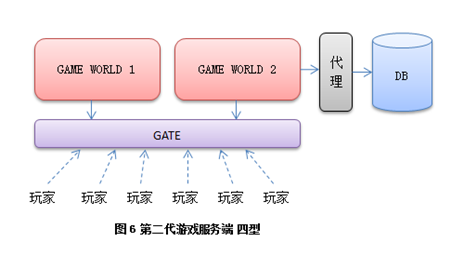
\includegraphics[width=8cm,clip]{gameServer6.png} 	
				\label{fig:gameServer6}
			\end{figure} 	
			\paragraph{尝试切分功能}把网络功能单独提取出来,让用户统一去连接一个网关服务器,再有网关服务器转发数据到后端游戏服务器。而游戏服务器之间数据交换也统一连接到网管进行交换。这样类型的服务器基本能稳定的为玩家提供游戏服务,一台网关服务1-2万人,后面的游戏服务器每台服务5k-1w,依游戏类型和复杂度不同而已,图中隐藏了很多不重要的服务器,如登录和管理。这是目前应用最广的一个模型,到今天任然很多新项目会才用这样的结构来搭建。
			
			人都是有惯性的,按照先前的经验,似乎把 MUDOS拆分的越开性能越好。于是大家继续想,网关可以拆分呀,基础服务如聊天交易,可以拆分呀,还可以提供web接口,数据库可以拆分呀,于是有了下面的模型,如图7。
			\begin{figure}[h] 	
				\centering
				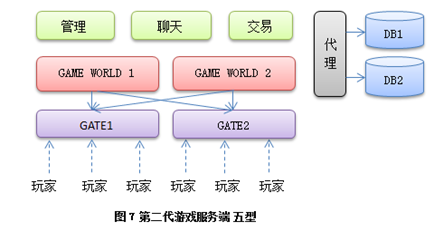
\includegraphics[width=8cm,clip]{gameServer7.png} 	
				\label{fig:gameServer7}
			\end{figure} 	
			
		\subsection{总结}上面这些类型基本都是从拆分 MUDOS开始,将 MUDOS中的各个部件从单机一步步拆成分布式。虽然今天任然很多新项目在用上面某一种类似的结构,或者自己又做了其他热点模块的拆分。
\newpage
\section{无缝世界地图}
		\subsection{用户特点}
			\begin{enumerate}[fullwidth,itemindent = 2em]
				\item  频繁的读取数据
				\item  在线人数多
				\item  利用在线数据进行游戏
				\item  无缝地图
			\end{enumerate}
			
			\begin{figure}[h] 	
				\centering
				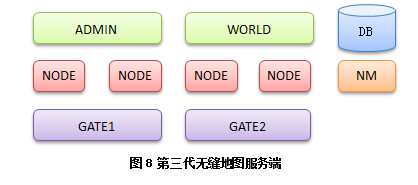
\includegraphics[width=8cm,clip]{gameServer8.png} 	
				\label{fig:gameServer8}
			\end{figure} 
		\subsection{具体细节}	
			\paragraph{地图管理}比较以往按照地图来切割游戏而言,无缝世界并不存在一块地图上面的人有且只由一台服务器处理了。
			每台 Node服务器用来管理一块地图区域,由 NodeMaster(NM)来为他们提供总体管理。更高层次的 World则提供大陆级别的管理服务。这里省略若干细节服务器,比如传统数据库前端,登录服务器,日志和监控等,统统用 ADMIN概括
			
			\paragraph{用户与地图 到 用户与节点}玩家从一块区域走向另外一块区域需要简单处理一下,如图9.玩家1完全由节点A控制,玩家3完全由节点B控制。而处在两个节点边缘的2号玩家,则同时由A和B提供服务。玩家2从A移动到B的过程中,会同时向A请求左边的情况,并向B请求右边的情况。但是此时玩家2还是属于A管理。直到玩家2彻底离开AB边界很远,才彻底交由B管理。按照这样的逻辑将世界地图分割为一块一块的区域,交由不同的 Node去管理
			
			  \begin{figure}[h] 	
			 	 \centering
				 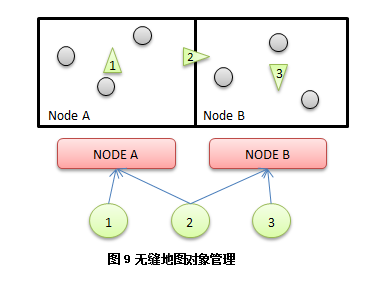
\includegraphics[width=8cm,clip]{gameServer9.png} 	
				 \label{fig:gameServer9}
			   \end{figure} 
			   
			\paragraph{节点与用户的逻辑复杂化解决模型}于是碰到第一个问题是很多 Node服务器需要和玩家进行通信,需要问管理服务器特定UID为多少的玩家到底在哪台 Gate上,以前按场景切割的服务器这个问题不大,问了一次以后就可以缓存起来了,但是现在服务器种类增加不少,玩家又会飘来飘去,按UID查找玩家比较麻烦;另外一方面 GATE需要动态根据坐标计算和哪些 Node通信,导致逻辑越来越厚,于是把:“用户对象”从负责连接管理的 GATE中切割出来势在必行于是有了下面的模型,如图10.
			
				\begin{figure}[h] 	
					\centering
					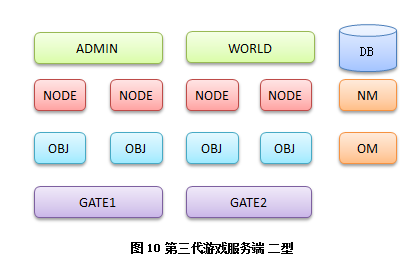
\includegraphics[width=8cm,clip]{gameServer10.png} 	
					\label{fig:gameServer10}
				\end{figure} 
			网关服务器再次退回到精简的网络转发功能,而用户逻辑则由按照 UID划分的 OBJ服务器来承担,GATE是按照网络接入时的负载来分布,而 OBJ则是按照资源的编号(UID)来分布,这样和一个用户通信直接根据 UID计算出 OBJ服务器编号发送数据即可。而新独立出来的 OBJ则提供了更多高层次的服务:
				\begin{itemize}
					\item  对象移动:管理具体玩家在不同的 Node所管辖的区域之间的移动,并同需要的 Node进行沟通。
					\item  数据广播:Node可以给每个用户设置若干 TAG,然后通知 Object Master 按照TAG广播。
					\item  对象消息:通用消息推送,给某个用户发送数据,直接告诉 OBJ,不需要直接和 GATE打交道。
					\item  好友聊天:角色之间聊天直接走 OBJ/OBJ MASTER
				\end{itemize}
				
			\paragraph{负载问题}整个服务器主体分为三层以后,NODE专注场景,OBJ专注玩家对象,GATE专注网络。这样的模型在无缝场景服务器中得到广泛的应用。但是随着时间的推移,负载问题也越来越明显,做个活动,远来不活跃的区域变得十分活跃,靠每周维护来调整还是比较笨重的,于是有了动态负载均衡。
			
					\subparagraph{动态负载均衡方案1:按照负载切分管理地图}由 Node Master 定时动态移动修改一下各个 Node的边界,而不同的玩家对象按照先前的方法从一台 Node上迁移到另外一台 Node上。这样 Node Master定时查找地图上的热点区域,计算新的场景切割方式,然后告诉其他服务器开始调整,具体处理方式还是和上面对象跨越边界移动的方法一样,如图11.
						\begin{figure}[h] 	
					     	\centering
							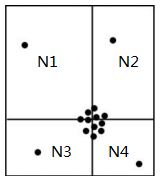
\includegraphics[width=8cm,clip]{gameServer11.png} 	
							\label{fig:gameServer11}
				    	\end{figure} 
				
					\subparagraph{动态负载均衡方案2:按照负载使用多节点服务}将地图按照标准尺寸均匀切割成静态的网格,每个格子由一个具体的Node负责,但是根据负载情况,能够实时的迁移到其他 Node上。在迁移分为三个阶段:准备,切换,完成。三个状态由Node Master负责维护。准备阶段新的 Node开始同步老 Node上面该网格的数据,完成后告诉NM;NM确认OK后同时通知新旧 Node完成切换。完成切换后,如果 Obj服务器还在和老的 Node进行通信,老的 Node将会对它进行纠正,得到纠正的 OBJ将修正自己的状态,和新的 Node进行通信。如图12.
				
						\begin{figure}[h] 	
							\centering
							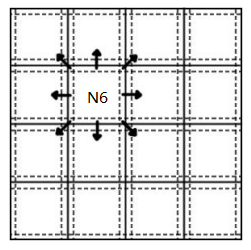
\includegraphics[width=8cm,clip]{gameServer12.png} 	
							\label{fig:gameServer12}
						\end{figure} 
    	\subsection{总结}	从无缝地图引入了分布式对象模型开始,已经完全脱离 MUDOS体系,成为一种新的服务端模型。又由于动态负载均衡的引入,让无缝服务器如虎添翼,容纳着超过上一代游戏服务器数倍的人数上限,并提供了更好的游戏体验,我们称其为第三代游戏服务端架构。网游以大型多人角色扮演为开端,RPG网游在相当长的时间里一度占据90\%以上,使得基于 MMORPG的服务端架构得到了蓬勃的发展
    	
\newpage
\section{局域网游戏服务器}
		\subsection{用户特点}
		\begin{enumerate}[fullwidth,itemindent = 2em]
			\item  频繁的读取数据
			\item  每局游戏一般都是 8人以内
			\item  利用在线数据进行游戏
			\item  全国只有一套服务器
			\item  玩家和玩家之使用 P2P的方式连接在一起
			\item  无缝地图
		\end{enumerate}
		
		\begin{figure}[h] 	
			\centering
			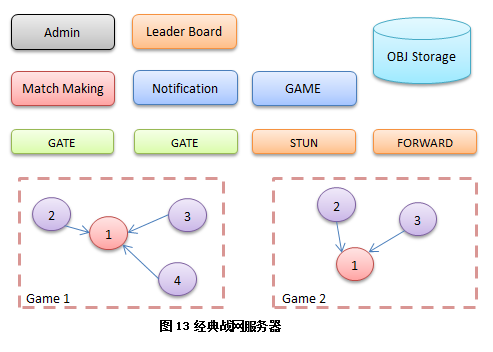
\includegraphics[width=8cm,clip]{gameServer13.png} 	
			\label{fig:gameServer13}
		\end{figure} 
		
		
		\subsection{具体细节}
			\paragraph{游戏匹配}玩家通过 Match Making 服务器使用:创建、加入、自动匹配、邀请 等方式组成一局游戏。服务器会选择一个人做 Host,其他人 P2P连接到做主的玩家上来。STUN是帮助玩家之间建立 P2P的牵引服务器,而由于 P2P联通情况大概只有 75\%,实在联不通的玩家会通过 Forward进行转发。
			
			\paragraph{数据流}大量的连接对战,体育竞技游戏采用类似的结构。P2P有网状模型(所有玩家互相连接),和星状模型(所有玩家连接一个主玩家)。复杂的游戏状态在网状模型下难以形成一致,因此星状P2P模型经受住了历史的考验。除去游戏数据,支持语音的战网系统也会将所有人的语音数据发送到做主的那个玩家机器上,通过混音去重再编码的方式返回给所有用户。
			
			\paragraph{游戏同步问题}激烈的游戏过程必然带来到较 RPG复杂的多的同步策略,这样的同步机制往往带来的是很多游戏结果由客户端直接计算得出,那在到处都是破解的今天,如何保证游戏结果的公正呢?
			主要方法就是投票法,所有客户端都会独立计算,然后传递给服务器。如果结果相同就更新记录,如果结果不一致,会采取类似投票的方式确定最终结果。同时记录本剧游戏的所有输入,在可能的情况下,找另外闲散的游戏客户端验算整局游戏是否为该结果。并且记录经常有作弊嫌疑的用户,供运营人员封号时参考。
			
		\subsection{总结}本套服务器设备类似于CS1.5与CS1.6中的局域网对战系统,选择一个主机作为host.其他连接完成游戏。这类游戏安全方面不好控制,但确实存在很多这样的游戏开发体系,如果存在商城盈利模式,感觉还是这个不合适。
		
\newpage
\section{总体分析章}
	\subsection{分解功能}在游戏服务器中,可以看出存在着一种单一职责的开发趋向, 将每一种功能逐渐隔离, 逐渐细化,然后走向分布式,这利于开发,也利于性能。
	
	\subsection{具体实例}
	\begin{figure}[h] 	
		\centering
		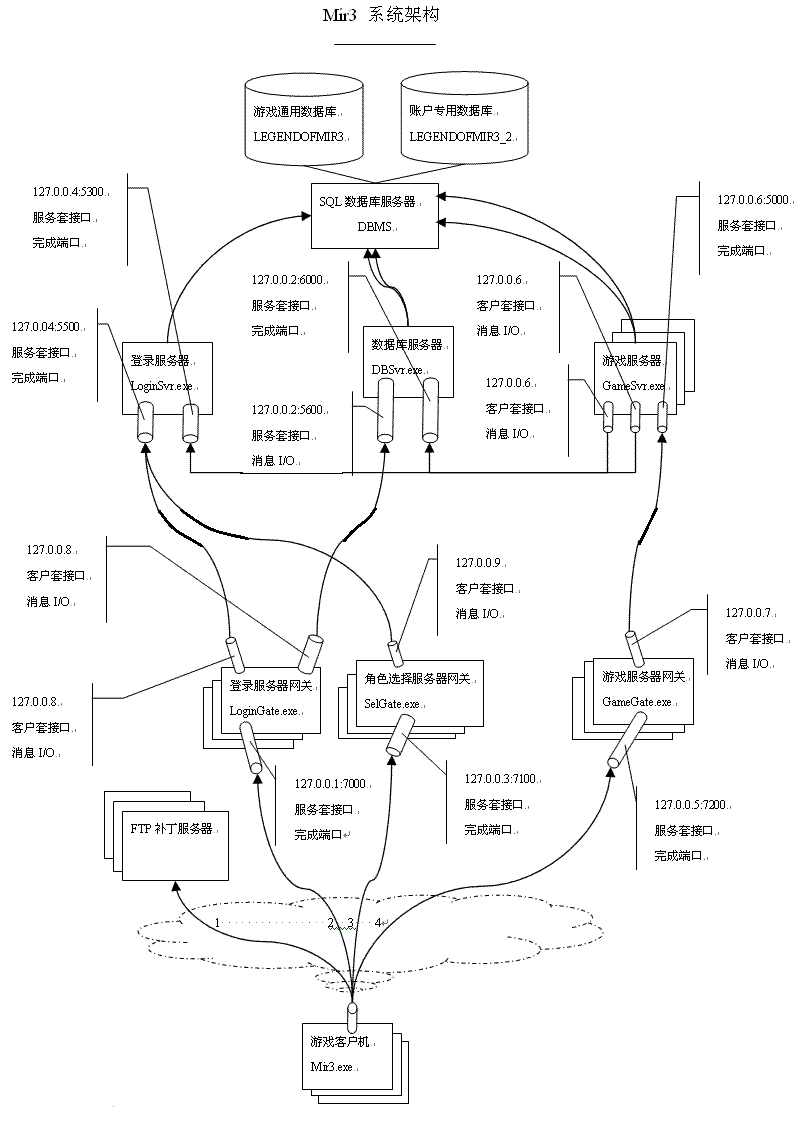
\includegraphics[width=14cm,clip]{gameServer14.png} 	
		\label{fig:gameServer14}
	\end{figure} 


\section{项目学习获取}
		\begin{figure}[h] 	
			\centering
			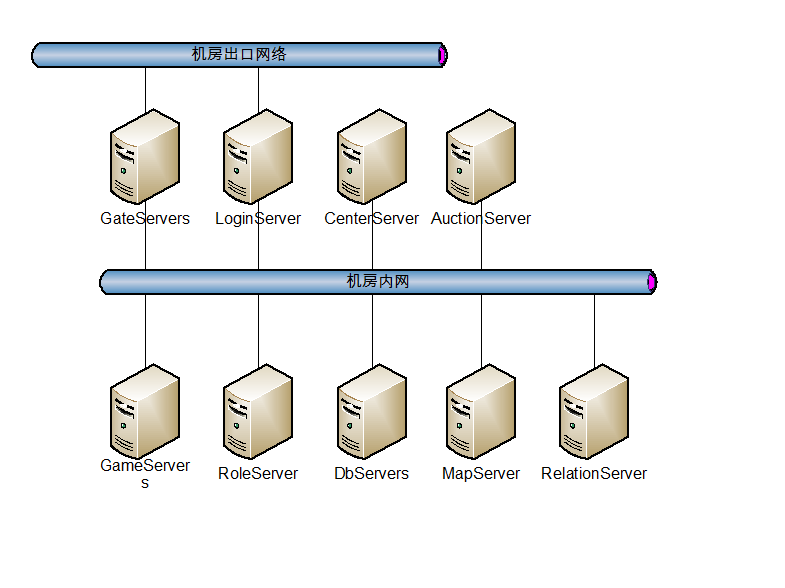
\includegraphics[width=14cm,clip]{gameServer15.png} 	
			\label{fig:gameServer15}
		\end{figure} 	
		
		
		\begin{figure}[h] 	
			\centering
			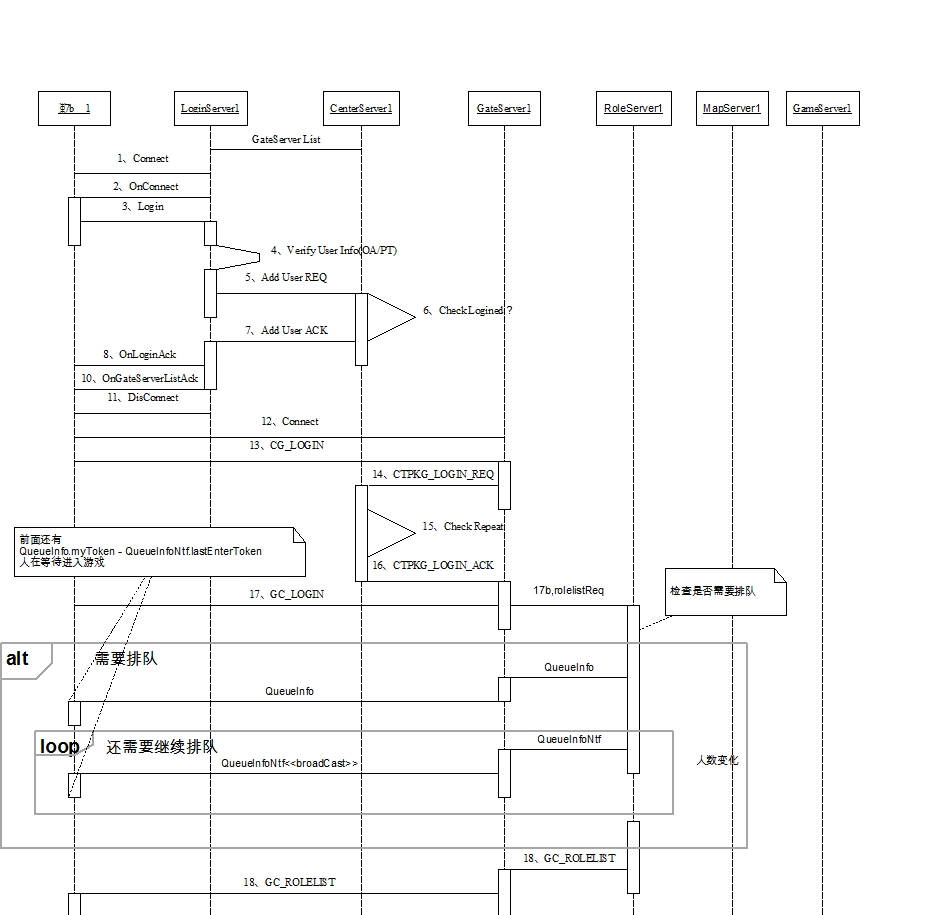
\includegraphics[width=14cm,clip]{gameServer16.png} 	
			\label{fig:gameServer16}
		\end{figure} 					
\end{document} 
 		    